\documentclass[sigconf]{acmart}
\usepackage[utf8]{inputenc}
\copyrightyear{2020}
\acmYear{2020}
\setcopyright{iw3c2w3}
\acmConference[WWW '20 Companion]{Companion Proceedings of the Web Conference 2020}{April 20--24, 2020}{Taipei, Taiwan}
\acmBooktitle{Companion Proceedings of the Web Conference 2020 (WWW '20 Companion), April 20--24, 2020, Taipei, Taiwan}
\acmPrice{}
\acmDOI{10.1145/XXXXXX.XXXXXX}
% Authors, replace the red X's with your assigned DOI string during the rightsreview eform process.
\acmISBN{978-1-4503-7024-0/20/04}

\settopmatter{printacmref=true}
\begin{document}

\title{From Fugu With Love: New Capabilities for the Web}

\author{Thomas Steiner}
\email{tomac@google.com}
\affiliation{%
  \institution{Google Germany GmbH}
  \streetaddress{ABC-Str. 19}
  \city{Hamburg}
  \postcode{20354}
  \country{Germany}
}

\author{Pete LePage}
\email{petele@google.com}
\affiliation{%
  \institution{Google LLC}
  \streetaddress{111 8th Avenue}
  \city{New York}
  \state{NY}
  \postcode{10011}
  \country{United States}
}

\author{Thomas Nattestad}
\email{nattestad@google.com}
\author{Rory McClelland}
\email{rorymcclelland@google.com}
\affiliation{%
  \institution{Google Germany GmbH}
  \streetaddress{Erika-Mann-Str. 33}
  \city{Munich}
  \postcode{80636}
  \country{Germany}
}

\author{Alex Russell}
\email{slightlyoff@google.com}
\affiliation{%
  \institution{Google LLC}
  \streetaddress{345 Spear Street}
  \city{San Francisco}
  \state{CA}
  \postcode{94105}
  \country{United States}
}

\author{Dominick Ng}
\email{dominickn@google.com}
\affiliation{%
  \institution{Google Australia}
  \streetaddress{48 Pirrama Road}
  \city{Sydney}
  \state{NSW}
  \postcode{2009}
  \country{Australia}
}

\renewcommand{\shortauthors}{Thomas Steiner, Pete LePage, Thomas Nattestad, \textit{et al.}}

\begin{abstract}
We present a greeting card web application that is useful in all modern browsers,
but sees its experience progressively enhanced through new and upcoming browser capabilities
such as native file system access, system clipboard access, contacts retrieval,
periodic background sync, screen wake lock, web sharing features, and more.
\end{abstract}

\begin{CCSXML}
<ccs2012>
<concept>
<concept_id>10002951.10003260.10003282</concept_id>
<concept_desc>Information systems~Web applications</concept_desc>
<concept_significance>500</concept_significance>
</concept>
<concept>
<concept_id>10002951.10003260.10003300.10003302</concept_id>
<concept_desc>Information systems~Browsers</concept_desc>
<concept_significance>500</concept_significance>
</concept>
</ccs2012>
\end{CCSXML}

\ccsdesc[500]{Information systems~Web applications}
\ccsdesc[500]{Information systems~Browsers}

\keywords{Progressive Web Apps, Web \textsc{api}s, Web Incubator Community Group}

\maketitle

\section{Introduction and Background}

\subsection{The App Gap}

Modern web browsers support impressive web applications far beyond
the web's origin as a global space of linked documents.
WebAssembly (Wasm) is enabling new classes of games and productivity apps,
Web Real-Time Communication (Web\textsc{rtc}) enables new ways to communicate,
and service workers allow developers to create reliably fast web experiences
almost regardless of network conditions.
However, there are some capabilities, like file system access,
raw clipboard access, background app refresh, and more,
that are available to native desktop and mobile platforms,
but that are not available to the web platform.
These missing capabilities mean some types of apps cannot be delivered on the web,
or that these apps are less useful.
In colloquial terms, this is sometimes referred to as the \textit{app gap}.

\subsection{Using Web Technologies, But Not the Web}

The app gap causes some developers to simply not build for the web.
However, doing this often means focusing on only one platform,
or using more complex toolchains.
Frameworks such as Apache Cordova\footnote{Apache Cordova:
\url{https://cordova.apache.org/}} (mobile)
and Electron\footnote{Electron: \url{https://electronjs.org/}} (desktop)
allow developers to build apps \textit{using} web technologies,
but also to access more of the underlying capabilities of the device
than are available on the broader web platform.
This approach leverages the web's interoperability and relative ease of development,
but it comes with security challenges~\cite{carettoni17,luo11},
and requires that users pay the cost of downloading and storing an entire web runtime per app.

\subsection{The Capabilities Project, Or Project Fugu}

The Capabilities Project (or Project Fugu) aims to bridge this gap.
We want to enable the web to access native app capabilities
\textit{without} having to compromise user security, privacy, or trust,
or having to package entire app runtimes.
Giving developers these new tools will empower the open web
as a place where almost any experience can be created,
and make it a~first class platform for developing apps that run on any browser,
with any operating system, and on any device.
We design and develop these new capabilities in an open and transparent way
in the \textsc{w3c}'s Web Incubator Community
Group\footnote{\textsc{wicg}: \url{https://wicg.io/}} (\textsc{wicg})
using the existing open web platform standards processes
while getting early feedback from developers and other browser vendors
as we iterate on the design of these features to ensure its interoperability.

This work is a~cross-company effort, with contributors from Google, Microsoft, and Intel.
The monthly meetings are open to join upon invitation
and have shared notes,\footnote{Project Fugu notes:
\url{https://bit.ly/fugu-sync}}
accessible to anyone in the Chromium organization.

We have identified and prioritized an initial set of capabilities
we heard partner demand for and that we see as critical to closing the gap
between web and native.
People interested in the list can review it by searching the Chromium bug database
for bugs that are tagged with the label
\texttt{proj-fugu}.\footnote{Project Fugu bugs: \url{https://bit.ly/fugu-bugs}}
Regarding the project's code name: fugu is a pufferfish that is considered a delicacy, however,  
if not carefully prepared, it can be lethally poisonous. 
This analogy works quite well with many of the capabilities we deal with.
We have outlined our vision for a~more capable web in a~blog post~\cite{lepage18}
on the Chromium blog and invite interested parties to follow along the project's progress
on the dedicated project landing
page.\footnote{Project Fugu landing page:
\url{https://developers.google.com/web/updates/capabilities}}

\subsection{The Capabilities Process}

We have developed a process to make it possible to design and develop
new web platform capabilities that meet the needs of developers quickly,
in the open, and most importantly, without moving feature development outside the standards process.
The capabilities process, depicted in \autoref{fig:fuguprocess}, consists of the following steps:

\begin{enumerate}
  \item \textbf{Identify the developer need:}
  
  The first step is to identify and understand the developer need.
  How are they doing it today? And what and whose problems or frustrations
  are fixed by this new capability? Typically, these come in as feature request
  from developers, frequently via bugs filed on \url{bugs.chromium.org}.

  \item \textbf{Create an explainer:}

  After identifying the need for a new capability, create an explainer,
  essentially a~design document that is meant to explain the problem,
  along with sample code showing how the \textsc{api} might work.
  The explainer is a living document that will go through heavy iteration
  as the new capability evolves.

  \item \textbf{Get feedback and iterate on the explainer:}

  Once the explainer has a reasonable level of clarity,
  it is time to publicize it, to solicit feedback, and iterate on the design.
  This is an opportunity to verify the new capability meets the needs of developers
  and works as expected and to gather public support and verify
  that there really is a need for this.

  \item \textbf{Move the design to a specification and iterate:}
  
  Once the explainer is in a good state,
  the design work transitions into a formal specification,
  working with developers and other browser vendors to iterate and improve on the design.
  Once the design starts to stabilize, we typically use an
  origin trial\footnote{Origin Trial: \url{http://googlechrome.github.io/OriginTrials/explainer.html}}
  to experiment with the implementation.
  Origin trials allow developers to try new features with real users,
  and give feedback on the implementation.

  \item \textbf{Ship it:}

  Finally, once the origin trial is complete, the spec has been finalized,
  and all of the other launch steps have been completed, it is time to ship it to stable.  
\end{enumerate}

It is worth noting that many ideas never make it past an explainer or origin trial stage.
\textit{Not} shipping a feature because it does not solve the developer need is fine.
We want to highlight that this process does \textit{not} replace the Blink launch
process;\footnote{Blink launch process: \url{https://www.chromium.org/blink/launching-features}}
both go hand in hand.

\begin{figure}[htb]
  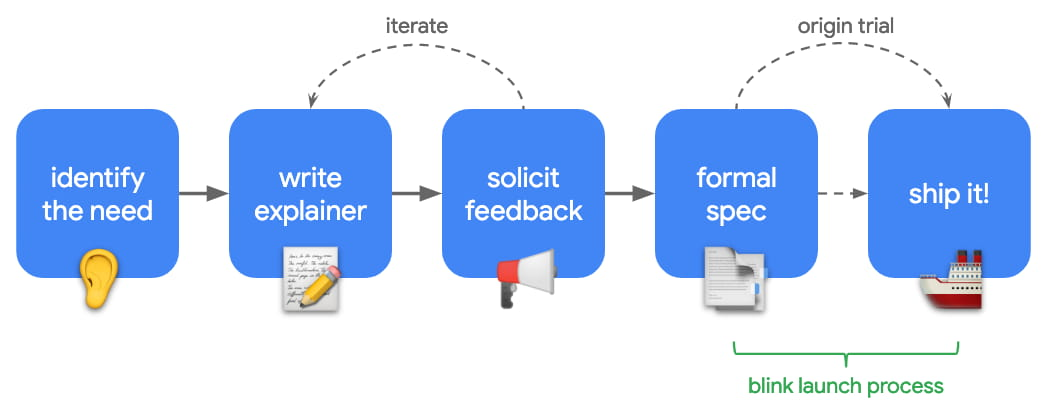
\includegraphics[trim={0 0.5cm 0 0},clip,width=0.925\columnwidth]{capabilities-process.jpg}
  \caption{The Capabilities Process}
  \label{fig:fuguprocess}
  \vspace{-0.65em}
\end{figure}

\subsection{Permissions}

Some of the capabilities we work on are potentially harmful for users
if not handled appropriately (we recall the code name of this project).
In a~position paper~\cite{russell18} presented at the \textsc{w3c} Permissions Workshop,
we have outlined our standpoints regarding evolving the current permission model.
We propose the following steps:

\begin{itemize}
  \item Permission-requesting \textsc{api}s need to introduce the ability for
    developers to register interest in a~capability before ever being allowed to prompt users
    and to be called back when the situation changes, \textit{e.g.},\
    if increased site engagement is noted, when before the threshold would not have been reached.
  \item Since different web \textsc{api}s currently have disparate ways to signal
    a~developer's intent to use them, permissions requests should be centralized
    on a~single method~\cite{yasskin17} to enable
    better user controls and bring much needed developer consistency.
  \item The Permissions \textsc{api}~\cite{lamouri19} should be extended with a revoke method,
    so developers are able to ensure their applications operate with least-privilege.
  \item The Web Application Manifest should be extended to include fields
    which allow sites to identify to the runtime a maximum set of permissions.
    Requests for permissions not included in this list should fail.
\end{itemize}

\subsection{Access to Powerful Web Platform Features}

Allowing users to control which sites are able to access powerful \textsc{api}s
is crucial for maintaining the security and privacy properties of the web.
The impact of restrictions on the developer ergonomics and user utility
of the \textsc{api} and the web platform overall must also be considered.
The following general principles~\cite{ng19} summarize the overall approach of the Chromium project
to evaluating how powerful new features should be controlled on the web:

\begin{itemize}
  \item Access to powerful APIs should be available to the entire web of secure contexts,
    with control managed exclusively by user consent \textsc{ux} like prompts or pickers at time-of-use.
  \item \textsc{api}-specific restrictions on the scope of access may also be used
    to guard against potential abuse.
  \item Usage of powerful \textsc{api}s should be clearly disclosed to users,
    ideally using a central hub that offers users control over what sites
    can use which capabilities.
  \item Installing a~web app is associated with persistence,
    and thus persistent and/or background access to powerful \textsc{api}s
    may only be granted (possibly subject to additional requirements) to installed web apps.
    Non-installed sites may still request and be granted permission to use powerful \textsc{api}s,
    but should not have their access persisted.
  \item Installation or engagement alone should not act as a vote of trust
    for either granting access or enabling the ability to ask for access to powerful \textsc{api}s.
    Separately, efforts should be made to curtail the existing persistency
    on the web platform outside of installed web apps, \textit{e.g.},\ time-limiting permission grants,
    more aggressively expiring cookies, and restricting background task execution.
\end{itemize}

\section{Prior Art}

This is not the first attempt at making the web a~powerful application platform.
We list three examples that went to market with this promise.
While there are more,\footnote{Others: Adobe \textsc{air}, Windows Hosted Apps,
Blackberry WebWorks apps, \textsc{w3c} Widgets} these three are very representative.

\subsection{Chrome Apps}

In 2013, Chrome Apps~\cite{kay13} promised to bring together the speed, security,
and flexibility of the modern web with the powerful functionality
previously only available with software installed on devices. 
Chrome Apps were designed to work offline, were capable of running in stand-alone windows,
could be launched directly from the desktop,
supported desktop notifications,
and could interact with \textsc{usb}, Bluetooth and other devices connected to a~desktop,
including digital cameras.
They were kept updated automatically and synced their state to the cloud.
Chrome Apps could use a~set of proprietary \texttt{chrome.*}
\textsc{api}s.\footnote{\texttt{chrome.*}
\textsc{api}s: \url{https://developer.chrome.com/apps/api_index}}
After three years, Chrome Apps were deprecated in August
2016.\footnote{Chrome Apps deprecation:
\url{http://bit.ly/chrome-apps-deprecation}}
Project Fugu is a~direct successor to Chrome Apps.
In fact, Progressive Web Apps built using Fugu \textsc{api}s
are one of the recommended migration
strategies.\footnote{Transitioning from Chrome Apps: \url{https://developers.chrome.com/apps/migration}}
Support for Chrome Apps in Chrome will end by June 2022.\footnote{Chrome Apps end of support:
\url{https://goo.gle/chrome-apps-support-end}}

\subsection{Palm web\textsc{OS}}

Palm web\textsc{OS}\footnote{Palm web\textsc{OS} announcement:
\url{http://bit.ly/palm-webos-announcement}}
was invented exclusively for mobile use.
It recognized that users wanted their people, calendars, and information to move with them,
wherever they were, wirelessly, as opposed to being bound to a personal computer.
At its core, web\textsc{OS} leverages industry-standard technologies,
including web technologies such as \textsc{css}, \textsc{xhtml}, and \textsc{js}.
It changed owners several times and lives on as an open-source
project\footnote{web\textsc{OS} open-source project: \url{https://www.webosose.org/}}
powering smart devices, \textit{e.g.},\ \textsc{tv}s.

\subsection{Firefox \textsc{OS}}

Firefox \textsc{OS}, also known as
Boot~2~Gecko\footnote{Boot to Gecko: \url{https://developer.mozilla.org/en-US/docs/Archive/B2G_OS}}
and first commercially released in 2013,
is a~discontinued open-source operating system
designed by Mozilla and external contributors.
It was based on the rendering engine of the Firefox web browser, Gecko,
and on the Linux kernel.
The operating system was capable of running web applications directly
or those installed from an app marketplace.
The applications used standards like \textsc{js} and \textsc{html}5,
and web \textsc{api}s that could communicate directly with the underlying hardware.
A~fork of Firefox \textsc{OS} now gains traction under the name of
Kai\textsc{OS},\footnote{Kai\textsc{OS}: \url{https://www.kaiostech.com/}}
especially on feature phones in emerging markets.

\section{Demo Description}

\subsection{Core Contributions and Intended Audience}

In March 2003, Nick Finck and Steve Champeon stunned the web design world
with the concept of progressive enhancement~\cite{champeon03},
a~strategy for web design that emphasizes core webpage content first,
and that then progressively adds more nuanced and technically rigorous layers
of presentation and features on top of the content.
While in 2003, progressive enhancement was about using at the time modern \textsc{css} features,
unobtrusive JavaScript, progressive enhancement in 2020 is about using modern browser capabilities.

We will present a~greeting card web application that is useful in all modern browsers,
but sees its experience progressively enhanced through new and upcoming browser capabilities
such as native file system access, system clipboard access, contacts retrieval,
periodic background sync, screen wake lock, web sharing features, and more.

The target audience are academia and industry web developers, browser engineers,
and people involved in the \textsc{w3c} standards process,
as well as web privacy researchers.

\subsection{Demo Link and Demo Requirements}

The demo is publicly available at \url{https://glitch.com/~fugu-greetings},
where it can either be explored directly,
or where its source code can be inspected and cloned.
We recommend running the demo in the latest Chrome
Canary\footnote{Chrome Canary: \url{https://www.google.com/chrome/canary/}}
or Edge
Canary\footnote{Edge Canary: \url{https://www.microsoftedgeinsider.com/en-us/download}}
browsers (both at version 82 as of February 2020).
Since this demo is about bleeding edge web \textsc{api}s,
some browser runtime flags need to be set (below, replace \texttt{chrome://}
with \texttt{edge://} on Edge):

\begin{itemize}
  \item \url{chrome://flags/#native-file-system-api}
  \item \url{chrome://flags/#enable-experimental-web-platform-features}  
  \item \url{chrome://flags/#periodic-background-sync}
\end{itemize}

\subsection{Baseline Application}

Progressive Web Applications (\textsc{pwa}s) are a type of application software
delivered through the web, built using common web technologies
including \textsc{html}, \textsc{css}, and \textsc{js}.
They are intended to work on any platform that uses a standards-compliant browser.
As such, we will start with a simple drawing web application
that serves as the baseline greeting card app that is offline-enabled,
can be added to the user's home screen, \textit{etc.},
and step-by-step add new browser capabilities
as progressive enhancements that are dynamically offered on supporting browsers.
We note that the currently rudimentary visual design of this application is \textit{not} focus of the demo.

\subsection{Native File System \textsc{api} Support}

Drawing everything from scratch is hard.
We thus add a~feature that allows the user to import a local image into the application.
\autoref{fig:file} shows the file import dialog where, after granting access,
the user can open a local image file and add it to their drawing.
Later, they can also save their creation to disk.
Both operations are enabled through the Native File System Access \textsc{api}~\cite{kruisselbrink19}
and not to be confused with legacy workarounds that required uploading a local file to a server
and downloading a~copy.

\begin{figure}[b]
  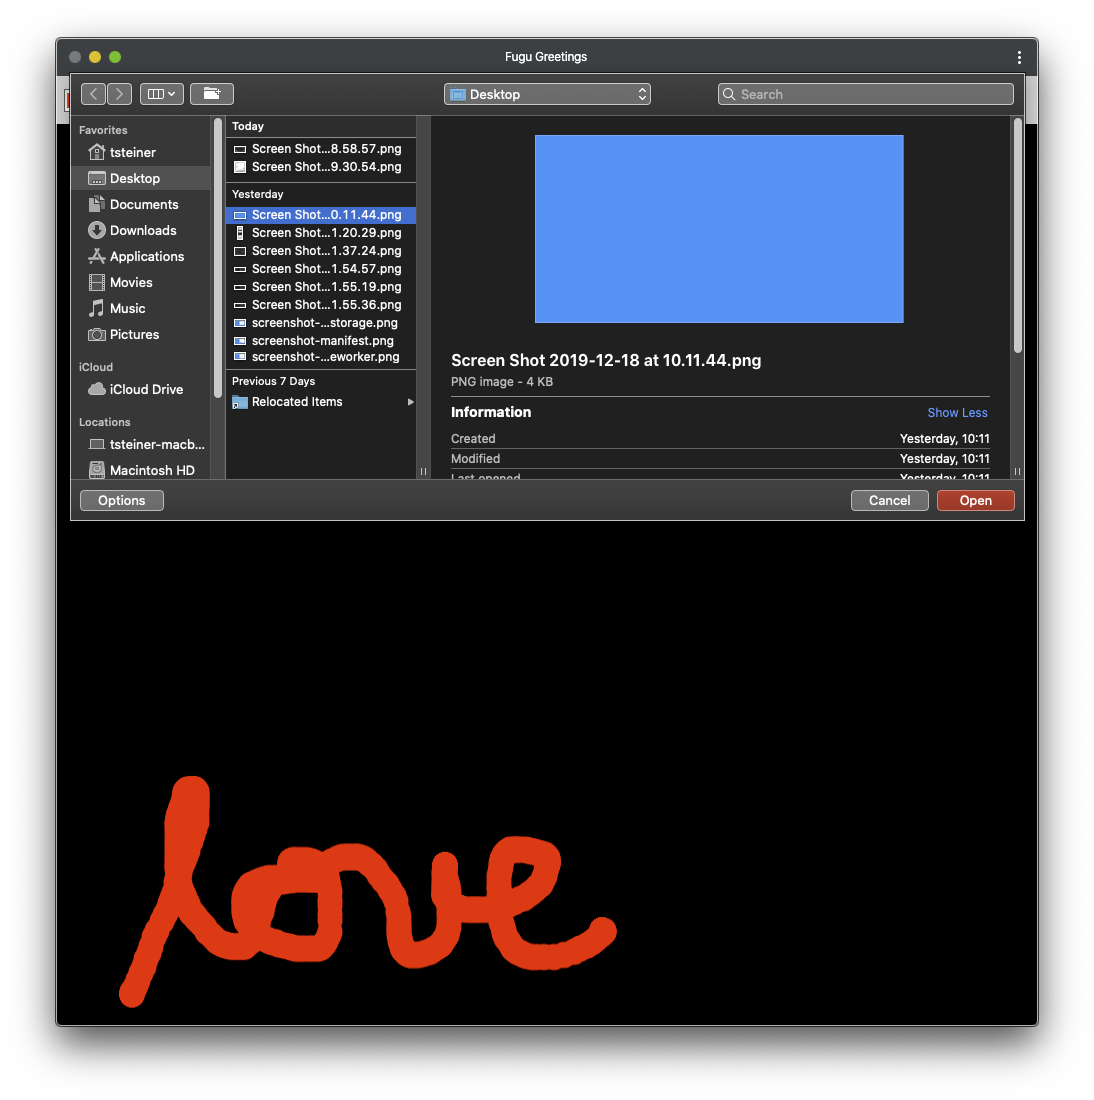
\includegraphics[width=0.75\columnwidth]{file.png}
  \caption{Native File System Access \textsc{api}}
  \label{fig:file}
\end{figure}

\subsection{Web Share (Target) \textsc{api} Support}

Creating an advanced greeting cards app is nonsensical if there is no one out to appreciate the cards.
We thus add a~feature that allows the user to share their drawings with the world.
The Web Share \textsc{api}~\cite{giuca2017webshare} allows for the sharing of files
using the native device's share mechanism.
\autoref{fig:share} shows the user initiating a~share of a drawing on an Android device.
Both the native Google Hangouts app as well as the native Facebook app offer itself
as share targets.
The other way round, through the Web Share Target \textsc{api},
the greeting card application itself can become a~share target
that one can share images to as card sources, for example, from the photo gallery app.

\begin{figure}[b]
  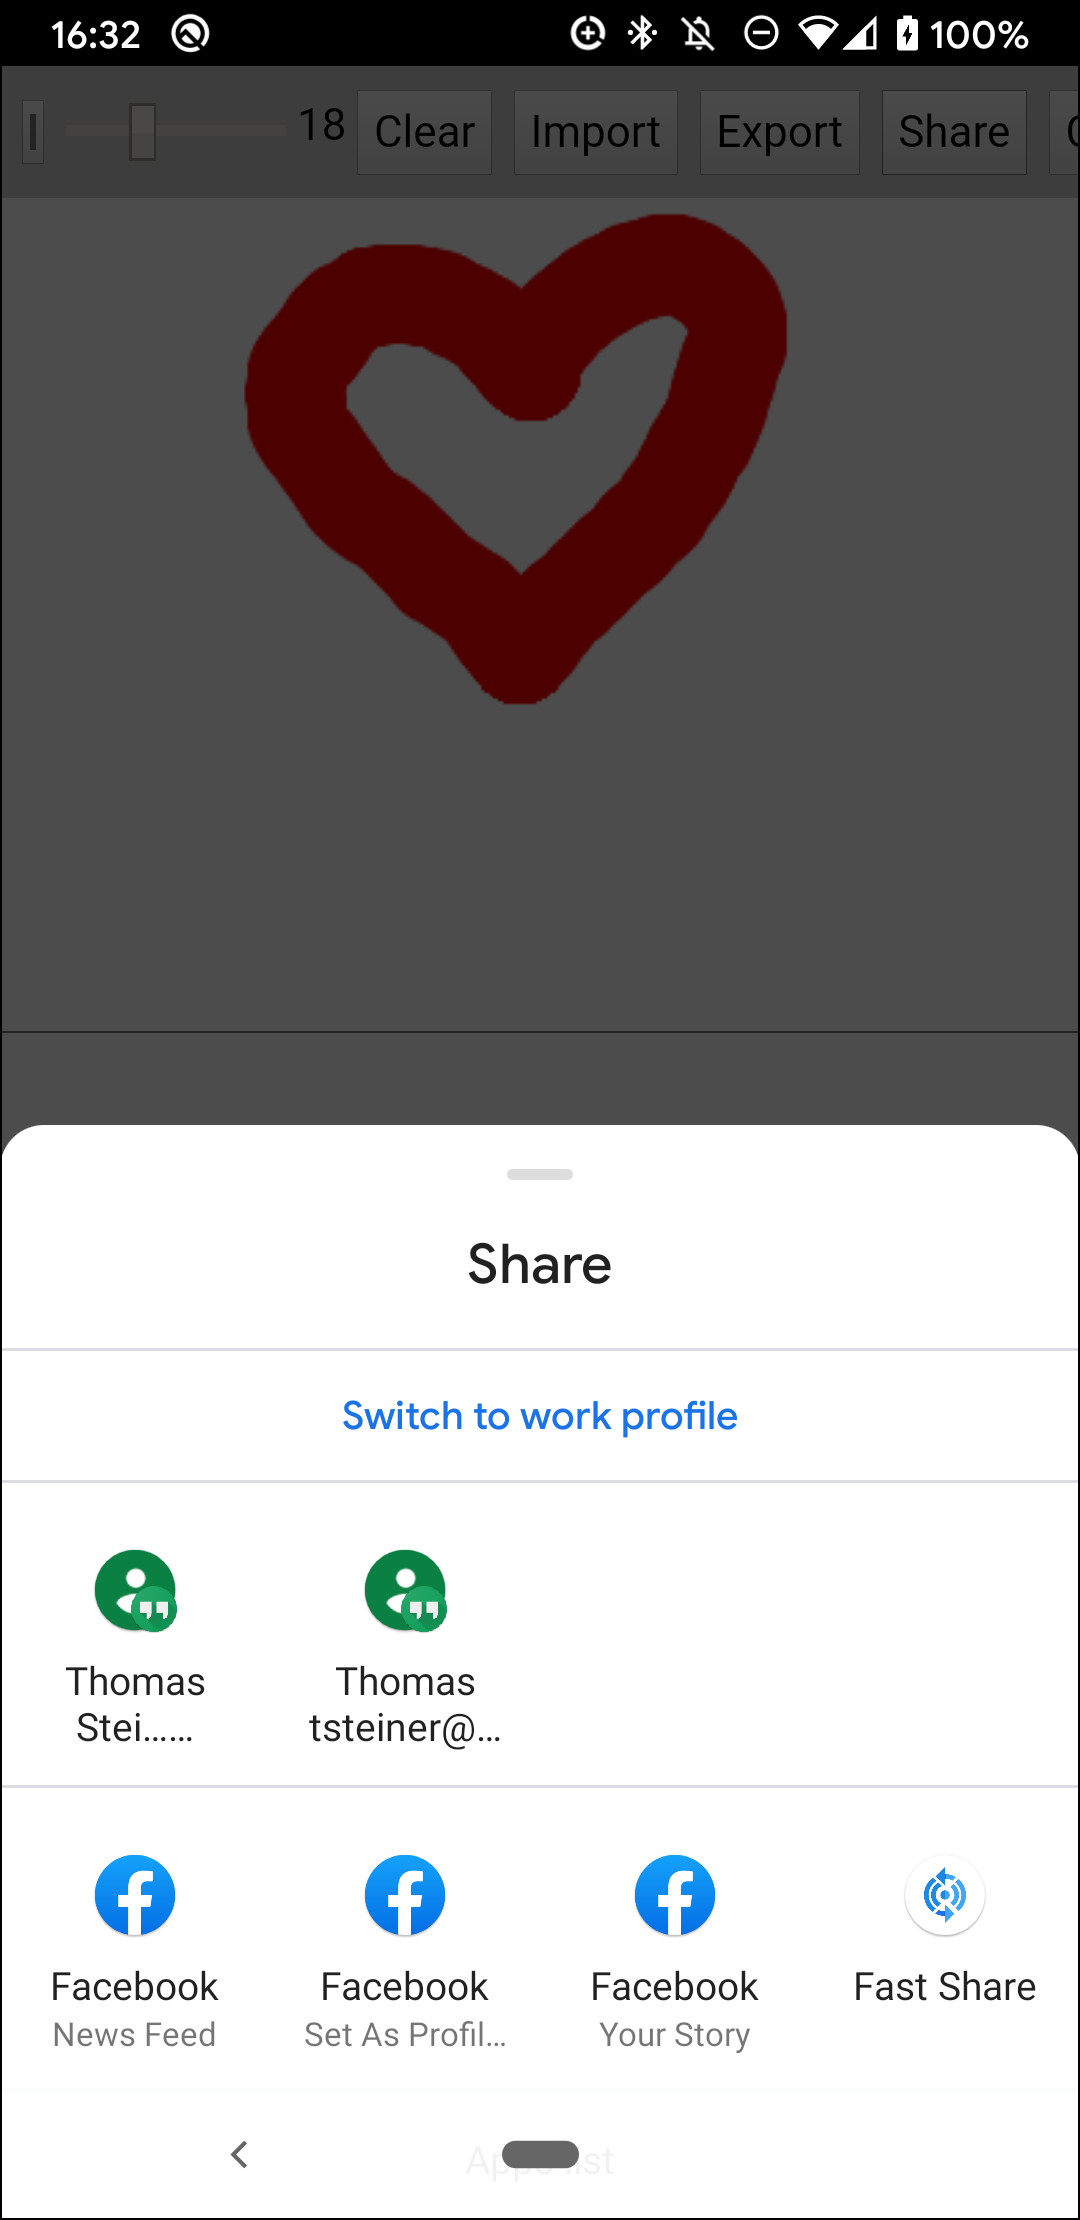
\includegraphics[width=0.4\columnwidth]{share.png}
  \caption{Web Share \textsc{api}}
  \label{fig:share}
\end{figure}

\subsection{Contact Access \textsc{api} Support}

At times it can be hard to correctly type a~greeting card recipient's name,
for example, when it is written in a~different script
that the present keyboard layout does not support.
We add a~feature that allows users to pick one (or multiple) of their local contacts
and add their names to the greeting card message.
This is a~one-off operation facilitated by the Contact Picker \textsc{api}~\cite{beverloo19};
no continuous contacts access is granted
and the user can choose the contact details.

\subsection{Clipboard \textsc{api} Support}

Occasionally users might want to paste a~picture from another app into the greeting card app,
or copy a drawing from the greeting card app into another app.
We add a~feature that allows users to copy and paste images from and to the app.
The Clipboard \textsc{api}~\cite{kacmarcik19} allows for the asynchronous copying and pasting
of image data (currently limited to Portable Network Graphics images).

\subsection{Badging \textsc{api} Support}

If the greeting cards app is installed on a~user's device,
it will have an icon on their home screen.
This icon can be used to convey fun information on the icon badge
like the number of brushstrokes a~given drawing has taken.
The Badging \textsc{api}~\cite{giuca19} enables apps to set a~numeric badge on the app icon
that increments with each stroke.

\subsection{Other \textsc{api}s Support}

The demo will showcase a number of other \textsc{api}s, namely the
Shape Detection \textsc{api} to detect shapes like faces,
the Wake Lock  \textsc{api} to keep the screen awake
while the user waits for drawing inspiration, 
the Periodic Background Sync  \textsc{api} to surprise the user
with a~new greeting card template each day,
the Idle Detection \textsc{api} to clear the greeting card
when the user is no longer interacting with the application
(for example, when it is running in a~kiosk setup),
and the File Handling \textsc{api}, which allows the app
to register as a~file handler to integrate with the operating system's file explorer.

\section{Conclusions}

We hope to gather feedback on these proposed features from the conference attendees,
as well as trigger conversations about future challenges around
permissions, security, and browser compatibility,
and invite interested parties to learn more about Project Fugu.

\bibliographystyle{ACM-Reference-Format}
\bibliography{fugu}

\end{document}
\endinput
